\chapter{Метрические пространства}

\section{Определение и примеры}

\begin{definition}
	$M$ -- множество, $\rho : M \times M \to \R$ \\
	$(M, \rho)$ -- метрическое пространство, если:
	\begin{enumerate}
		\item $\rho(x, y) \ge 0, \qquad \rho(x, y) = 0 \iff x = y $
		\item $\rho(x, y) = \rho(y, x)$
		\item $\rho(x, y) \le \rho(x, z) + \rho(z, y) $
	\end{enumerate}
\end{definition}

\begin{exmpls}
	\item $ \R, \quad \rho(x, y) = |x - y| $
	\item $ \R^2, \qquad \rho_2((x_1, y_1), (x_2, y_2)) = \sqrt{(x_1 - x_2)^2 + (y_1 - y_2)^2} $ -- обобщается до $\R^n$
	$$ \rho_1((x_1, y_1), (x_2, y_2)) = |x_1 - x_2| + |y_1 - y_2| $$
	$$ \rho_p ((x_1, y_1), (x_2, y_2)) = \bigg( |x_1 - x_2|^p + |y_1 - y_2|^p \bigg)^{\faktor1p}, \qquad p \ge 1 $$
	Каждая $\rho_p$ является метрикой. Свойтсва 1 и 2 очевидны. Проверим неравенство треугольника:
	\begin{proof}
		$$ \bigg( \sum_i |x_i + p_i|^p \bigg)^{\faktor1p} \le \bigg( \sum_i |x_i|^p \bigg)^{\faktor1p} + \bigg( \sum_i |y_i|^p \bigg)^{\faktor1p} $$
	\end{proof}
	$$ \rho_{\infty}((x_1, y_1), (x_2, y_2)) = \max\set{|x_1 - x_2|, |y_1 - y_2|} \text{ -- без доказательства} $$
	$\rho_1$ -- манхэтенская метрика (если в городе все улицы перпендикулярны ``осям'', то $\rho_1$ -- \textbf{любое} кратчайшее расстояние по улицам)
	\item $M$ -- множество
	$$ \rho(x, y) \define
	\begin{cases}
		1, \qquad x \ne y \\
		0, \qquad x = y
	\end{cases} $$
	$ B(x_0, \faktor12) = \set{x_0} $
	\item $(M, \rho)$ -- метрическое пространство
	$$ \rho'(x, y) \define \frac{\rho(x, y)}{1 + \rho(x, y)} \text{ -- тоже метрика} $$
	Теперь $\rho'(x, y) < 1 $
	$$ \rho''(x, y) = \max\set{\rho(x, y), 1} \text{ -- рассматриваем только расстояния, меньшие 1. Тоже метрика} $$
	\item $M$ -- множество строк из $0$ и $1$ длины $n$ \\
	$\rho(x, y)$ -- количество различных символов
	\begin{undefthm}{Задача}
		Есть строки из $n$ символов \\
		При передаче может возникнуть не более $k$ ошибок \\
		Посылаем сколько-то строк (часть из них искажается) \\
		Нужно, чтобы:
		\begin{itemize}
			\item Хотя бы одна строчка не исказилась
			\item Получатель мог однозначно определить, какая строчка не исказилась
		\end{itemize}
	\end{undefthm}
	\item $M$ -- пространство (хороших) функций на $[a, b]$
	$$ \rho_1(f, g) \define \int_a^b|f(x) - g(x)|dx $$
	У хороших функций такой интеграл точно существует (например, хорошими будут непрерывные)
	$$ \rho_2(f, g) \define \sqrt{ \int_a^b (f(x) - g(x))^2dx} $$
	$$ \rho_p(f, g) \define \bigg( \int_a^b |f(x) - g(x)|^pdx \bigg)^{\faktor1p} $$
	$$ \rho_\infty \define \sup |f(x) - g(x)|, \qquad x \in [a, b] $$
	\item $M$ -- множество (хороших) фигур на плоскости (например, многоугольников)
	$$ \rho(F, G) \define S_{F \triangle G} $$
	Метрика Хауссдорфа:
	\begin{itemize}
		\item Есть 2 кривые
		\item По одной из них движется поливальная машина (поливает кружочек вокруг себя, радиусом $\veps$)
		\item Хотим так подобрать $\veps$, чтобы вторая кривая была полностью полита
	\end{itemize}
	$$ ``\rho(F, G)" \define \inf\set{\veps | \forall x \in F \quad \exist y \in G : \rho(x, y) \le \veps} $$
	Очевидно, что такой $\veps$ не будет симметричным. Поэтому, берём максимум из них двоих:
	$$ \rho(F, G) \define \max\set{ \inf\set{\veps | \forall x \in F \quad \exist y \in G : \rho(x, y) \le \veps}, \inf\set{\veps | \forall x \in G \quad \exist y \in F : \rho(x, y) \le \veps} } $$
	\item $\Z$
	$$ |n| =
	\begin{cases}
		n, \qquad n \ge 0 \\
		-n, \qquad n < 0
	\end{cases} $$
	Возьмём $p \in \Prime$ \\
	Положим $||n|| = 2^{-v_p(n)} $, где $v_p(n)$ -- степень вхождения $p$ в $n$
	$$ v_p(\frac{m}n) \define v_p(m) - v_p(n) $$
	Таким образом, мы расширили $||\cdot||$ на $\Q$ \\
	$$ \rho_p(a, b) \define
	\begin{cases}
		||a - b||, \qquad a \ne b \\
		0, \qquad a = b
	\end{cases}, \qquad a, b \in \Q $$
	$ \rho_p $ -- $p$-адическая метрика
\end{exmpls}

Доказательство того, что это всё -- метрики, остаётся упражнением (хотя бы часть)

\begin{definition}
	Шар с центром $x_0$ и радиусом $\veps$:
	$$ B(x_0, \veps) \define \set{x \in M | \rho(x, x_0) < \veps} $$
\end{definition}

\begin{figure}[!ht]
	\begin{subfigure}{0.49\textwidth}
		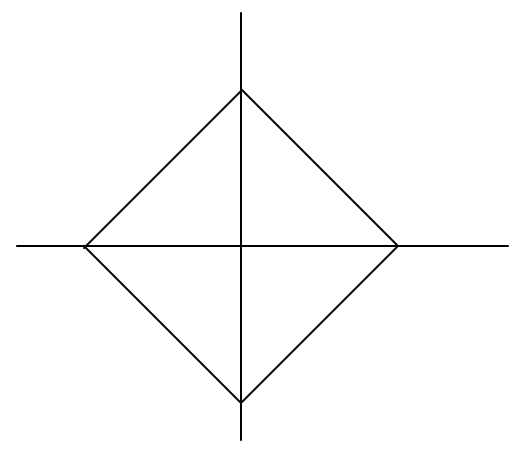
\includegraphics[width=\textwidth]{1}
		\caption{$\rho_1$}
	\end{subfigure}
	\begin{subfigure}{0.49\textwidth}
		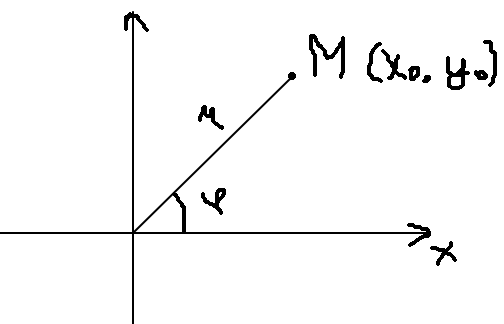
\includegraphics[width=\textwidth]{2}
		\caption{$\rho_\infty$}
	\end{subfigure}
	\caption{Шары по различным метрикам (из примера 2)}
\end{figure}

\section{Расположение точки относительно множества}

$ (M, \rho)$ -- метрическое пространство \\
$ A \sub M, \qquad x_0 \in M $

\begin{definition}
	$x_0$ называется внутренней для $A$, если $\exist \veps > 0 : B(x_0, \veps) \sub A $
\end{definition}

\begin{definition}
	$x_0$ называется внешней для $A$, если $\exist \veps > 0 : B(x_0, \veps) \cap A = \O $
\end{definition}

\begin{definition}
	Иначе $x_0$ -- граничная, то есть
	$$ \forall \veps > 0
	\begin{cases}
		B(x_0, \veps) \not\sub A \\
		B(x_0, \veps) \not\sub M \setminus A
	\end{cases} $$
\end{definition}

\begin{definition}
	Множество внутренних точек называется внутренностью ($\operatorname{Int}(A)$) \\
	Множество внешних точек называется внешностью ($\operatorname{Ex}(A)$) \\
	Множество граничных точек называется границей ($\delta A$, $\operatorname{Fr}(A)$)
\end{definition}

\begin{intuition}
	$ \operatorname{Int} (M \setminus A) = \operatorname{Ex} A $
\end{intuition}

\begin{definition}
	$ \operatorname{Cl} A \define \operatorname{Int} A \cup \delta A $ -- замыкание $A$
\end{definition}

\begin{definition}
	Множество $A$ называется открытым, если $A = \operatorname{Int} A $, то есть
	$$ \forall x_0 \in A \quad \exist \veps > 0 : B(x_0, \veps) \sub A $$
\end{definition}

\begin{definition}
	Множество $A$ называется замкнутым, если $A = \operatorname{Cl} A $, то есть $M \setminus A$ открыто
\end{definition}
